% Pengaturan ukuran teks dan bentuk halaman dua sisi
\documentclass[10pt,twoside]{report}

% Pengaturan ukuran halaman dan margin
\usepackage[a5paper,top=25mm,left=25mm,right=20mm,bottom=25mm]{geometry}

% Pengaturan ukuran spasi
\usepackage[singlespacing]{setspace}

% Judul dokumen
\title{Buku Laporan Kerja Praktik ITS}
\author{Musk, Elon Reeve \and Kjellberg, Felix Arvid Ulf}

% Pengaturan format bahasa
\usepackage[indonesian]{babel}

% Pengaturan detail pada file PDF
\usepackage[pdfauthor={\@author},bookmarksnumbered,pdfborder={0 0 0}]{hyperref}

% Pengaturan jenis karakter
\usepackage[utf8]{inputenc}

% Pengaturan ukuran indentasi paragraf
\setlength{\parindent}{2em}

% Pengaturan ukuran spasi paragraf
\setlength{\parskip}{0.5ex}

% Package lainnya
\usepackage{etoolbox} % Mengubah fungsi default
\usepackage{enumitem} % Pembuatan list
\usepackage{lipsum} % Pembuatan template kalimat
\usepackage{graphicx} % Input gambar
\usepackage{longtable} % Pembuatan tabel
\usepackage[table,xcdraw]{xcolor} % Pewarnaan tabel
\usepackage[numbers]{natbib} % Kutipan artikel
\usepackage{eso-pic} % Pembuatan background
\usepackage{changepage} % Pembuatan teks kolom
\usepackage{wrapfig} % Wrapping gambar

% Definisi untuk "Hati ini sengaja dikosongkan"
\def\kosong{
  \vspace*{\fill}
  \begin{center}\textit{Halaman ini sengaja dikosongkan}\end{center}
  \vfill
}
\patchcmd{\cleardoublepage}{\hbox{}}{\kosong}{}{}

% Pengaturan penomoran halaman
\usepackage{fancyhdr}
\fancyhf{}
\renewcommand{\headrulewidth}{0pt}
\pagestyle{fancy}
\fancyfoot[CE,CO]{\thepage}
\patchcmd{\chapter}{plain}{fancy}{}{}
\patchcmd{\chapter}{empty}{plain}{}{}

% Pengaturan format judul bab
\usepackage{titlesec}
\titleformat{\chapter}[display]{\bfseries\Large}{BAB \centering\Roman{chapter}}{0ex}{\vspace{0ex}\centering}[\vspace{2ex}]
\titleformat{\section}{\bfseries\large}{\MakeUppercase{\thesection}}{1ex}{}
\titleformat{\subsection}{\bfseries\large}{\MakeUppercase{\thesubsection}}{1ex}{}
\titleformat{\subsubsection}{\bfseries\large}{\MakeUppercase{\thesubsubsection}}{1ex}{}
\titlespacing{\chapter}{0ex}{0ex}{2ex}
\titlespacing{\section}{0ex}{2ex}{1ex}
\titlespacing{\subsection}{0ex}{1ex}{0.5ex}
\titlespacing{\subsubsection}{0ex}{1ex}{0.5ex}

% Pengaturan persamaan
\newenvironment{conditions}
{\par\vspace{\abovedisplayskip}\noindent
  \tabularx{\columnwidth}{>{$}l<{$} @{${}={}$} >{\raggedright\arraybackslash}X}}
{\endtabularx\par\vspace{\belowdisplayskip}}

% Pengaturan format baris program
\usepackage{listings}
\definecolor{comment}{RGB}{0,128,0}
\definecolor{string}{RGB}{255,0,0}
\definecolor{keyword}{RGB}{0,0,255}
\lstdefinestyle{codestyle}{
  commentstyle=\color{comment},
  stringstyle=\color{string},
  keywordstyle=\color{keyword},
  basicstyle=\footnotesize\ttfamily,
  numbers=left,
  numberstyle=\tiny,
  numbersep=5pt,
  frame=lines,
  breaklines=true,
  prebreak=\raisebox{0ex}[0ex][0ex]{\ensuremath{\hookleftarrow}},
  showstringspaces=false,
  upquote=true,
  tabsize=2,
}
\lstset{style=codestyle}

% Isi keseluruhan dokumen
\begin{document}

% Nomor halaman pembuka dimulai dari sini
\pagenumbering{roman}

% Sampul luar
\AddToShipoutPictureBG*{
  \AtPageLowerLeft{
    % Ubah nilai berikut jika posisi horizontal background tidak sesuai
    \hspace{-3.5mm}

    % Ubah nilai berikut jika posisi vertikal background tidak sesuai
    \raisebox{0mm}{
      
\includegraphics[width=\paperwidth,height=\paperheight]{sampul/sampul-luar.png}
    }
  }
}

% Menyembunyikan nomor halaman
\thispagestyle{empty}

% Pengaturan margin untuk menyesuaikan konten sampul
\newgeometry{top=70mm,left=25mm,right=20mm,bottom=25mm}

\begin{flushleft}

  % Pengaturan jenis dan warna teks yang digunakan
  \sffamily\color{white}

  % Ubah penomoran buku berikut sesuai dengan yang ditentukan oleh departemen
  \noindent\textbf{KERJA PRAKTIK - TD123456}
  \vspace{4ex}

  % Ubah kalimat berikut sesuai dengan nama perusahaan tempat kerja praktik
  \noindent{\large \textbf{PT. NATIONAL AERONAUTICS AND SPACE ADMINISTRATION}} \\
  % Ubah tanggal berikut sesuai dengan waktu berlangsungnya kerja praktik
  \textbf{(03 Desember 2020 s/d 03 Januari 2021)}
  \vspace{6ex}

  % Ubah kalimat berikut sesuai dengan judul topik kerja praktik
  \noindent{\large \textbf{PEMBUATAN ROKET LUAR ANGKASA ANTI GRAVITASI UNTUK PT. NASA}}
  \vspace{6ex}

  \begin{adjustwidth}{-2mm}{}
    \begin{tabular}{lcp{0.7\linewidth}}
      % Ubah kalimat-kalimat berikut sesuai dengan nama dan NRP mahasiswa pertama
      \textbf{Elon Reeve Musk} & & \textbf{NRP 0123 20 4000 0001} \\
      % Ubah kalimat-kalimat berikut sesuai dengan nama dan NRP mahasiswa kedua
      \textbf{Felix Arvid Ulf Kjellberg} & & \textbf{NRP 0123 20 4000 0002} \\
    \end{tabular}
  \end{adjustwidth}
  \vspace{4ex}

  \noindent\textbf{Dosen Pembimbing} \\
  % Ubah kalimat berikut sesuai dengan nama dosen pembimbing
  \textbf{Nikola Tesla, S.T., M.T.}
  \vspace{10ex}

  % Ubah kalimat berikut sesuai dengan nama departemen
  \noindent\textbf{DEPARTEMEN TEKNIK DIRGANTARA} \\
  % Ubah kalimat berikut sesuai dengan nama fakultas
  \textbf{Fakultas Teknologi Dirgantara} \\
  \textbf{Institut Teknologi Sepuluh Nopember} \\
  % Ubah kalimat berikut sesuai dengan tempat dan tahun pembuatan buku
  \textbf{Surabaya 2021}

\end{flushleft}

\restoregeometry

\cleardoublepage

% Sampul dalam
\AddToShipoutPictureBG*{
  \AtPageLowerLeft{
    % Ubah nilai berikut jika posisi horizontal background tidak sesuai
    \hspace{-3.5mm}

    % Ubah nilai berikut jika posisi vertikal background tidak sesuai
    \raisebox{0mm}{
      
\includegraphics[width=\paperwidth,height=\paperheight]{sampul/sampul-dalam.png}
    }
  }
}

% Pengaturan margin untuk menyesuaikan konten sampul
\newgeometry{top=70mm,left=25mm,right=20mm,bottom=25mm}

\begin{flushleft}

  % Pengaturan jenis teks yang digunakan
  \sffamily

  % Ubah penomoran buku berikut sesuai dengan yang ditentukan oleh departemen
  \noindent\textbf{MAGANG A - EC184918}\\
  \noindent\textbf{MAGANG B - EC184919}
  \vspace{4ex}

  % Ubah kalimat berikut sesuai dengan nama perusahaan tempat kerja praktik
  \noindent{\large \textbf{Google Bangkit}} \\
  % Ubah tanggal berikut sesuai dengan waktu berlangsungnya kerja praktik
  \textbf{(03 Mei 2021 s/d 09 Juni 2021)}
  \vspace{6ex}

  % Ubah kalimat berikut sesuai dengan judul topik kerja praktik
  \noindent{\large \textbf{Deteksi Kekerasan Otomatis Dalam Ruangan}}
  \vspace{6ex}

  \begin{adjustwidth}{-2mm}{}
    \begin{tabular}{lcp{0.7\linewidth}}
      \textbf{Aufa Nabil Amiri} &  & \textbf{NRP 0721 17 4000 0029} \\
    \end{tabular}
  \end{adjustwidth}
  \vspace{4ex}

  \noindent\textbf{Dosen Pembimbing} \\
  % Ubah kalimat berikut sesuai dengan nama dosen pembimbing
  \textbf{Reza Fuad Rachmadi ST., MT., Ph.D}
  \vspace{10ex}

  % Ubah kalimat berikut sesuai dengan nama departemen
  \noindent\textbf{DEPARTEMEN TEKNIK KOMPUTER} \\
  % Ubah kalimat berikut sesuai dengan nama fakultas
  \textbf{Fakultas Teknologi Elektro dan Informatika Cerdas } \\
  \textbf{Institut Teknologi Sepuluh Nopember} \\
  % Ubah kalimat berikut sesuai dengan tempat dan tahun pembuatan buku
  \textbf{Surabaya 2021}

\end{flushleft}

\restoregeometry

\cleardoublepage

% Lembar pengesahaan untuk departemen
\begin{center}
  {\Large \textbf{LEMBAR PENGESAHAN}}
  \vspace{6ex}

  \addcontentsline{toc}{chapter}{LEMBAR PENGESAHAN (DEPARTEMEN)}

  % Ubah kalimat berikut sesuai dengan judul topik kerja praktik
  {\large \textbf{Deteksi Kekerasan Otomatis Dalam Ruangan}}
  \vspace{6ex}

  Laporan Magang ini disusun untuk memenuhi persyaratan akademik Departemen Teknik Komputer - Fakultas Teknologi Elektro dan Informatika Cerdas - Institut Teknologi Sepuluh Nopember

  \vspace{2ex}

  % Ubah kalimat-kalimat berikut sesuai dengan tempat dan tanggal pengesahan
  Tempat Pengesahan di: Surabaya \\
  Tanggal: 16 Juni 2021
  \vspace{8ex}

  Menyetujui, \\
  Dosen Pembimbing,
  \vspace{12ex}

  % Ubah kalimat-kalimat berikut sesuai dengan nama dan NIP dosen pembimbing
  \textbf{\underline{Reza Fuad Rachmadi ST., MT., Ph.D}} \\
  NIP. 19850403 201212 1 001
  \vspace{8ex}

  Mengetahui, \\
  % Ubah kalimat berikut sesuai dengan jabatan kepala departemen
  Kepala Departemen Teknik Komputer FTEIC - ITS,
  \vspace{12ex}

  % Ubah kalimat-kalimat berikut sesuai dengan nama dan NIP kepala departemen
  \textbf{\underline{Dr. Supeno Mardi Susiki Nugroho, ST.,MT.}} \\
  NIP 19700313 199512 1 001

\end{center}

\cleardoublepage

% Lembar pengesahan untuk perusahaan
\begin{center}
  {\Large \textbf{LEMBAR PENGESAHAN}}
  \vspace{6ex}

  \addcontentsline{toc}{chapter}{LEMBAR PENGESAHAN (PERUSAHAAN)}

  % Ubah kalimat berikut sesuai dengan judul topik kerja praktik
  {\large \textbf{Deteksi Kekerasan Otomatis Dalam Ruangan}}
  \vspace{6ex}

  % Ubah kalimat berikut sesuai dengan kalimat pengesahan yang ditentukan oleh departemen
  Diajukan Guna Memenuhi Sebagian Persyaratan Kurikulum Fakultas Teknologi Elektro dan Informatika Cerdas Program Sarjana Pada Departemen Teknik Komputer Institut Teknologi Sepuluh Nopember
  \vspace{2ex}

  % Ubah kalimat-kalimat berikut sesuai dengan tempat dan tanggal pengesahan
  Tanggal: 21 Juni 2021

  \vspace{8ex}

  Mengetahui, \\
  Kepala Program Google Bangkit
  \vspace{12ex}

  % Ubah kalimat berikut sesuai dengan nama pembimbing perusahaan
  \textbf{\underline{Adrianus Yoza Aprilio}}
  \vspace{8ex}

  Mengetahui, \\
  % Ubah kalimat berikut sesuai dengan jabatan kepala perusahaan
  Pembimbing Program \textit{Capstone} Google Bangkit
  \vspace{12ex}

  % Ubah kalimat berikut sesuai dengan nama kepala perusahaan.
  \textbf{\underline{Dian Ayuningtyas}}

  \vspace{8ex}

\end{center}

\cleardoublepage

% Kata pengantar
\begin{center}
  \Large\textbf{KATA PENGANTAR}
\end{center}
\vspace{2ex}

\addcontentsline{toc}{chapter}{KATA PENGANTAR}

Puji syukur atas kehadirat Tuhan yang Maha Esa, karena atas rahmat dan karunia-Nya penulis telah dapat menyelesaikan magang di Google Bangkit yang dilaksanakan tanggal 1 Mei 2021 sampai dengan 09 Juni 2021. Dalam penyelesaian Laporan Magang ini, kami mengucapkan terimakasih kepada berbagai pihak yang telah membantu dalam penyelesaian laporan ini :

\begin{itemize}
  \item Bapak Dr. Supeno Mardi Susiki Nugroho, ST.,MT. selaku Kepala Departemen Teknik Komputer FTEIC-ITS
  \item Dr. Diah Puspito Wulandari, S.T.,M.Sc. selaku Koordinator Kerja Praktek Departemen Teknik Komputer ITS
  \item Dian Ayuningtyas sebagai mentor sekaligus pembimbing selama melakukan proses magang.
\end{itemize}

Magang merupakan kredit mata kuliah opsional yang digunakan sebagai konversi dalam Google Bangkit. Magang juga berfungsi sebagai pendalaman mahasiswa dalam pengaplikasian ilmu yang didapat pada saat perkuliahan ke dalam dunia kerja. Penulis menyampaikan permohonan maaf jika selama pelaksanaan magang terdapat hal yang kurang berkenan dan jikalau ada salah dalam penulisan laporan ini.

\begin{flushright}
  \begin{tabular}[b]{c}
    % Ubah kalimat berikut sesuai dengan tempat, bulan, dan tahun penulisan
    Surabaya, Juni 2021
    \\
    \\
    \\
    \\
    Penulis
  \end{tabular}
\end{flushright}

\cleardoublepage

% Daftar isi
\renewcommand*\contentsname{DAFTAR ISI}
\addcontentsline{toc}{chapter}{\contentsname}
\tableofcontents
\cleardoublepage

% Daftar gambar
\renewcommand*\listfigurename{DAFTAR GAMBAR}
\addcontentsline{toc}{chapter}{\listfigurename}
\listoffigures
\cleardoublepage

% Daftar tabel
\renewcommand*\listtablename{DAFTAR TABEL}
\addcontentsline{toc}{chapter}{\listtablename}
\listoftables
\cleardoublepage

% Nomor halaman isi dimulai dari sini
\pagenumbering{arabic}

% Bab 1 pendahuluan
% Ubah kalimat sesuai dengan judul dari bab ini
\chapter{PENDAHULUAN}

% Ubah konten-konten berikut sesuai dengan yang ingin diisi pada bab ini

\section{Latar Belakang}

Kekerasan merupakan kata yang berasal dari bahasa Latin \textit{violentus} yang berarti berkuasa atau kekuasaan. Secara arti, kekerasan merupakan sebuah ekspresi baik yang dilakukan secara fisik ataupun secara verbal yang mencerminkan pada tindakan agresi dan penyerangan pada kebebasan seseorang.

Menurut data yang didapat dari Komisi Nasional (Komnas) Perempuan, terdapat lebih dari 8000 kasus yang sudah ditangani hanya dalam kurun waktu tahun 2020 saja. Dan yang lebih parah lagi, apabila dibandingkan dengan tahun sebelumnya, terjadi kenaikan sebesar 60\%  kasus. Jumlah tersebut hanya menghitung jumlah kasus yang tercatat dan diketahui, namun, menurut perkiraan Komnas Perempuan, masih banyak sekali kasus yang tidak tercatat dan diketahui karena meningkatnya jumlah kuesioner yang dikembalikan, padahal kuesioner sendiri merupakan alat bantu yang cukup vital untuk mengetahui kondisi lingkungan sekitar pada seorang perempuan atau anak.

Hal yang sama juga terjadi di dalam sekolah. Data dari unicef menunjukkan bahwa pada tahun 2018, hampir 41\% anak pada umur 15 tahun pernah mengalami perundungan atau yang biasa disebut \textit{bullying}. Mirisnya, perundungan tidak hanya terbatas dilakukan oleh sesama siswa, namun tidak jarang juga dilakukan oleh guru.

Ditambah lagi dengan kondisi pandemi seperti sekarang ini, banyak sekali orang yang beraktifitas dari rumah, dan karena perubahan yang begitu tiba - tiba, banyak membuat orang menjadi stress dan tertekan. Imbasnya, semakin meningkatkan kemungkinan terjadinya kekerasan di dalam ruangan.

Salah satu hal yang paling menyulitkan dalam menangani kekerasan pada perempuan dan anak adalah karena seringnya, kekerasan dilakukan di area tertutup sehingga tidak diketahui oleh orang lain. Tidak jarang juga korban kekerasan banyak yang tidak mau melapor kepada petugas yang terkait, hal ini dibuktikan dengan banyaknya kuesioner Komnas Perempuan yang dikembalikan.

Sebagai mahasiswa departemen Teknik Komputer, saya berupaya merealisasikan sebuah sistem yang bernama Jaga Bersama. Jaga Bersama adalah sebuah sistem \textit{monitoring} cerdas yang dapat mendeteksi apabila terjadi suatu kekerasan, terkhusus kekerasan di dalam ruangan. Diharapkan dengan terealisasikannya sistem kami, maka dapat membantu untuk mengurangi angka kekerasan pada perempuan dan anak di Indonesia nantinya.


\section{Tujuan}

Tujuan dari magang ini dapat dilihat dari dua
sudut pandang sebagai berikut:

\vspace{0.5ex}

\begin{enumerate}[nolistsep]

      \item \textit{Secara Umum}
            \vspace{0.5ex}

            \begin{enumerate}[nolistsep]
                  \item Terciptanya suatu hubungan yang sinergis dan terarah antara dunia
                        perguruan tinggi dan dunia kerja sebagai pengguna outputnya.

                  \item Membuka wawasan mahasiswa agar dapat mengetahui dan memahami
                        aplikasi ilmunya di dunia industri.

                  \item Mahasiswa dapat mampu mengadakan pendekatan masalah secara utuh.

                  \item Menciptakan pola berpikir konstruktif yang
                        lebih berwawasan bagi mahasiswa.

            \end{enumerate}

            \vspace{0.5ex}

      \item \textit{Secara Khusus}
            \vspace{0.5ex}

            \begin{enumerate}[nolistsep]
                  \item Memperdalam pengetahuan mahasiswa dengan mengenal dan juga mempelajari
                        secara langsung mengenai pengolahan \textit{mobile application development} dan IoT secara umum.

                  \item Mengembangkan pengetahuan, sikap, keterampilan, kemampuan profesi melalui
                        penerapan ilmu, latihan kerja, dan pengamatan teknik yang akan diterapkan.
            \end{enumerate}

\end{enumerate}

\section{Bentuk Kegiatan}

Dalam proses magang, kami melaksanakan di rumah masing - masing (\textit{Work From Home}) dikarenakan program yang dilakukan di seluruh Indonesia secara serentak sehingga memang harus dilakukan secara jarak jauh melalui media Google Meet.

Pembuatan sistem kami kerjakan sesuai dengan \textit{timeline} yang sudah kami sepakati dan kami mengerjakan sesuai peran masing - masing. Adapun bentuk teknis kegiatannya adalah sebagai berikut :

\begin{enumerate}[nolistsep]
      \item Penyusunan laporan sementara yang dilakukan pada minggu terakhir kegiatan
            magang dilaksanakan. Selanjutnya laporan sementara ini dimintakan persetujuan
            kepada pembimbing magang yang bersangkutan. Dalam memberikan persetujuan
            terhadap laporan sementara ini maka pembimbing lapangan memberikan penilaian terhadap
            pelaksanaan magang yang dilaksanakan oleh mahasiswa. Laporan sementara ini
            selanjutnya dijadikan dasar untuk pembuatan laporan resminya. Penilaian dari pembimbing
            lapangan akan diserahkan pada dosen pembimbing magang di Departemen Teknik
            Komputer - ITS Surabaya.

      \item Penilaian kedua diberikan berdasarkan hasil penyusunan laporan resmi yang dibuat
            oleh mahasiswa selesai dilaksanakannya magang.

      \item Penilaian ketiga diberikan berdasarkan hasil presentasi laporan resmi magang.
\end{enumerate}

\section{Waktu dan Tempat Pelaksanaan}

Berikut tempat dan waktu pelaksanaan magang yang dilakukan pada :

\begin{tabular}{c l}
      Tempat & : Rumah Masing - Masing (WFH)  \\
      Waktu  & : 03 Mei 2021 s/d 09 Juni 2021
\end{tabular}

\section{Metodologi Magang}

Metodologi magang yang digunakan dalam pelaksanaan magang ini adalah sebagai berikut :

\begin{enumerate}[nolistsep]

      \item \textbf{Tahap Persiapan}

            Membuat \textit{timeline} beserta proposal untuk kemudian akan dicek dan diberi kritik atau saran oleh tim Bankgit.

      \item \textbf{Pengembangan Sistem}

            Sistem dikembangkan sesuai ide awal yang sudah tertulis di dalam proposal yang sudah disetujui. Selain itu juga dilakukan \textit{mentoring} dengan orang - orang dari industri.

      \item \textbf{Pembuatan Laporan}

            Pembuatan laporan yang dibutuhkan sebagai prasayarat kelulusan dalam mata kuliah magang.

\end{enumerate}

\section{Sistematika Penulisan}

Laporan Kerja Praktek ini terdiri atas lima bab dengan rincian sebagai berikut :
\vspace{0.5ex}

\begin{enumerate}[nolistsep]

      \item \textbf{Bab I Pendahuluan}
            \vspace{0.5ex}

            Pada BAB I dibahas mengenai latar belakang, tujuan, waktu dan tempat
            pelaksanaan Kerja Praktek, metode penulisan, serta sistematika penulisan.
            \vspace{0.5ex}

      \item \textbf{Bab II Profil Google Bangkit}
            \vspace{0.5ex}

            Pada BAB II dibahas mengenai profil singkat dari program Google Bangkit.
            \vspace{0.5ex}

      \item \textbf{Bab III Tinjauan Pustaka}
            \vspace{0.5ex}

            Pada BAB III dibahas mengenai teori-teori penunjang dalam pembuatan produk aplikasi,
            seperti \textit{mobile application}, adobe XD, \textit{firebase} dan \textit{App Engine}.
            \vspace{0.5ex}

      \item \textbf{Bab IV Desain dan Implementasi}
            \vspace{0.5ex}

            Pada BAB IV dibahas mengenai pembuatan produk.

            \vspace{0.5ex}

      \item \textbf{Bab V PENUTUP}
            \vspace{0.5ex}

            Pada BAB V dibahas mengenai kesimpulan dan saran.
            \vspace{0.5ex}

\end{enumerate}
\cleardoublepage

% Bab 2 profil perusahaan
% Ubah kalimat sesuai dengan judul dari bab ini
\chapter{PROFIL PROGRAM GOOGLE BANGKIT}

% Ubah konten-konten berikut sesuai dengan yang ingin diisi pada bab ini

\section{Sejarah Google Bangkit}

Google Bangkit adalah sebuah program yang digagas oleh google. Diawali pada tahun 2020 dengan berisi 300 peserta, Google Bangkit berhasil meraih perhatian banyak orang termasuk, menteri pendidikan saat ini, yaitu Nadiem Makarim. Banyak sekali alumni - alumninya yang mengatakan bahwa dengan mengikuti program Google Bangkit ini, mereka mendapatkan prospek kerja yang lebih baik sehingga meningkatkan kemungkinan untuk mendapatkan pekerjaan.

Pada tahun 2021 ini, Google Bangkit menerima peserta dengan jumlah yang jauh lebih banyak, yaitu sebesar 3000 peserta. Berbeda dengan Google Bangkit pada tahun 2020, tahun ini terdapat 3 fokusan yang dapat dipilih oleh peserta, terdapat \textit{Google Cloud Engineer}, \textit{Android Engineer} dan \textit{Machine Learning Engineer}. Tidak berhenti sampai disana, saat ini Google Bangkit berkerja sama dengan 15 partner universitas dan bahkan berkolaboasi dengan perusahan - perusahaan \textit{unicorn} seperti Gojek, Tokopedia, dan Traveloka.

Tentu saja disini sebagai suatu perusahaan yang sangat ternama, Google tidak hanya mengambil peserta dari kota - kota besar. Menurut William Florence, Pemimpin \textit{Asia Pacific Education Program}, bahwa terdapat 3000 peserta yang berasal dari 250 universitas dari segala penjuru Indonesia.  Selain itu, terdapat 30\% peserta perempuan, yang apabila dibandingkan dengan tahun lalu, terjadi peningkatan sebesar 4\%.

\section{Tujuan Google Bangkit}

Tujuan utama dari program Google Bangkit yang utama adalah meningkatkan kualitas manusia Indonesia sehingga menjadi manusia yang kreatif, terampil dan ahli dalam bidangnya masing - masing.

Selain itu, melalui program ini, diharapkan mahasiswa dapat membangun kepercayaan diri dalam berekreasi. Hal ini termasuk dengan kemampuan bertindak dan kerangka pikir kewirausahaan agar dapat mengatasi tantangan global dan membangun masa depan yang lebih baik.

Dan apabila kita melihat lebih dalam apa saja yang disuguhkan oleh Google Bangkit, dapat dilihat bahwa mahasiswa juga diharapkan untuk mengasah ketrampilan penting yang bermanfaat dalam dunia kerja, seperti \textit{design thinking}, kepemimpinan, serta kemampuan komunikasi dan presentasi.



\cleardoublepage

% Bab 3 tunjauan pustaka
% Ubah kalimat sesuai dengan judul dari bab ini
\chapter{TINJAUAN PUSTAKA}

% Ubah konten-konten berikut sesuai dengan yang ingin diisi pada bab ini

\section{Roket Luar Angkasa}

% Contoh input gambar dengan format *.jpg
\begin{figure} [ht] \centering
  % Nama dari file gambar yang diinputkan
  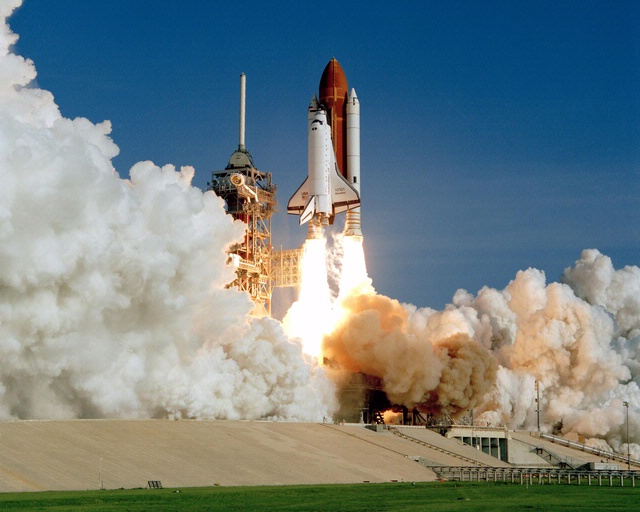
\includegraphics[scale=0.3]{gambar/space-shuttle.jpg}
  % Keterangan gambar yang diinputkan
  \caption{Peluncuran pesawat luar angkasa Discovery \citep{DiscoverySpaceShuttle}}
  % Label referensi dari gambar yang diinputkan
  \label{fig:SpaceShuttle}
\end{figure}

Roket luar angkasa merupakan \lipsum[16][1-10]

% Contoh penggunaan referensi dari gambar yang diinputkan
\emph{Discovery}, Gambar \ref{fig:SpaceShuttle}, merupakan \lipsum[17][1-9]

\section{Gravitasi}

Gravitasi merupakan \lipsum[18][1-10]

\subsection{Hukum Newton}

% Contoh penggunaan referensi dari pustaka
Newton \citep{Newton1687} pernah merumuskan bahwa \lipsum[19]
% Contoh penggunaan referensi dari persamaan
Kemudian menjadi persamaan seperti pada persamaan \ref{eq:FirstNewtonLaw}.

% Contoh pembuatan persamaan
\begin{equation}
  % Label referensi dari persamaan yang dibuat
  \label{eq:FirstNewtonLaw}
  % Baris kode persamaan yang dibuat
  \sum \mathbf{F} = 0\; \Leftrightarrow\; \frac{\mathrm{d} \mathbf{v} }{\mathrm{d}t} = 0.
\end{equation}

\subsection{Anti Gravitasi}

Anti gravitasi merupakan \lipsum[20]

\cleardoublepage

% Bab 4 desain dan implementasi
% Ubah kalimat sesuai dengan judul dari bab ini
\chapter{DESAIN DAN IMPLEMENTASI}

% Ubah konten-konten berikut sesuai dengan yang ingin diisi pada bab ini

\section{Deskripsi Sistem}

Sistem kami bernama JagaBersama, suatu sistem yang dapat digunakan untuk mendeteksi kekerasan baik itu merupakan kekerasan dalam rumah tangga maupun \textit{bullying} atau perundungan yang biasa terjadi di sekolah - sekolah maupun di tempat umum. Dengan memanfaatkan salah satu cabang dalam pembelejaran mesin yaitu \textit{Deep Learning} ditambah dengan pengolahan citra modern, kita dapat melakukan pendeteksian secara otomatis dengan cepat dan murah. Diharapkan dengan adanya sistem kami maka dapat mengurangi jumlah kasus kekerasan di Indonesia dan dapat memberikan suatu ide pendekatan yang baru dalam menanggulangi kekerasan di Indonesia.

Terdapat 2 target pengguna dalam sistem kami, yang pertama adalah Pengguna Umum yang akan memasang sistem kami (kamera + \textit{raspberry pi}) yang akan dapat secara otomatis mendeteksi kekerasan. Kemudian target pengguna yang pertama adalah Agen, agen disini yang dimaksud adalah agen yang dapat berasal dari Komnas Perempuan yang bertugas untuk menyelesaikan apabila terjadi suatu kasus kekerasan maupun bisa juga agen lain seperti polisi atau guru apabila kekerasan terjadi di sekolah.

Namun, sebagai catatan, tanggung jawab saya kebanyakan merupakan pada bagian membuat aplikasi Android yang digunakan sebagai antar-muka antar agen dengan sistem basis data secara keseluruhan.

\section{Implementasi Alat}

Terdapat 3 bagian terpisah dari sistem kami yang semuanya bekerja secara bersamaan sehingga menciptakan suatu sistem yang dapat berjalan dengan lancar dan \textit{reliable}. Bagian pertama adalah bagian \textit{Internet of Things} (IoT), selanjutnya adalah \textit{server} sebagai bagian paling penting dalam keseluruhan sistem dan terakhir adalah aplikasi Android sebagai antar-muka dengan agen. Gambar \ref{fig:framework} adalah gambaran secara luas bagaimana sistem kami bekeja secara keseluruhan.


\begin{figure} [!ht]
  \centering
  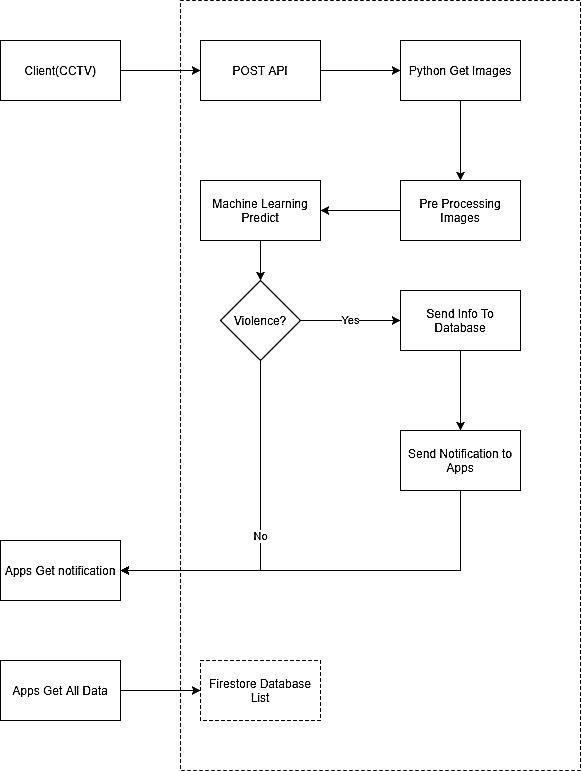
\includegraphics[width=0.8\textwidth]{gambar/framework.jpg}
  % Keterangan gambar yang diinputkan
  \caption{Diagram \textit{Framework} Keseluruhan Proyek}
  % Label referensi dari gambar yang diinputkan
  \label{fig:framework}
\end{figure}

\subsection{Implementasi IoT}
\cleardoublepage

% Bab 6 kesimpulan dan saran
% Ubah kalimat sesuai dengan judul dari bab ini
\chapter{KESIMPULAN DAN SARAN}

Pelaksanaan Magang dalam program Google Bangkit telah kami lakukan. Kami mendapatkan ilmu dan pengalaman bekerja dalam suatu proyek kolaborasi yang mengedepankan teknologi, kreativitas dan ketekunan dalam melakukan suatu hal. Dan juga dengan terlaksananya magang ini, kami mendapatkan pengetahuan baru tentang cara pengembangan suatu sistem dari awal sampai jadi dan dapat digunakan. Terkhusus, kami mendapatkan pengetahuan baru tentang bidang pembelajaran mesin, bidang pengembangan aplikasi Android, serta dalam bidang \textit{Cloud}. Tidak hanya bidang keilmuan yang sejalan dengan departemen kami saja, namun softskill seperti cara berpresentasi dan alur bekerja yang baik kami dapatkan saat magang kami berlangsung.

\section{Kesimpulan}

Berdasarkan kegiatan Magang yang sudah kami lakukan, diperoleh beberapa kesimpulan sebagai berikut :

\begin{enumerate}[nolistsep]

  \item Pembuatan sistem pendeteksi kekerasan ini dapat dilakukan dengan memanfaat beberapa teknologi seperti App Engine dan Firebase. Selain itu, untuk pembuatan aplikasi kami menggunakan bahasa Kotlin karena lebih mudah dalam proses membuat aplikasi dan memiliki hasil \textit{build} yang kecil, cepat dan ringan.

  \item Dengan menggunakan sistem Jaga Bersama, suatu tindak kejahatan berupa kekerasan dapat langsung terdeteksi secara otomatis dan seorang agen akan dapat dengan cepat mengetahui lokasi tempat kekerasan terjadi sehingga penanganan dapat lebih cepat dilakukan.

\end{enumerate}

\section{Saran}

Berdasarkan kegiatan Magang yang sudah kami lakukan, terdapat beberapa saran dari penulis yang dapat dijadikan masukan :

\begin{enumerate}[nolistsep]

  \item Adanya \textit{maintenance} yang berkala pada aplikasi untuk memastikan keseluruhan sistem dapat berjalan dengan semestinya.

  \item Memperbaiki tampilan agar aplikasi dapat lebih menarik bagi agen dan lebih mudah digunakan.

  \item Basis data yang digunakan sebaiknya menggunakan sistem yang lebih baik dan memiliki tingkat keamanan yang terjamin.

\end{enumerate}

\cleardoublepage

% Biografi penulis
\begin{center}
  \Large\textbf{BIOGRAFI PENULIS}
\end{center}
\vspace{2ex}

\addcontentsline{toc}{chapter}{BIOGRAFI PENULIS}

\begin{wrapfigure}{L}{0.3\textwidth}
  \centering
  \vspace{-3ex}
  % Ubah nama file gambar berikut dengan nama file foto dari mahasiswa pertama
  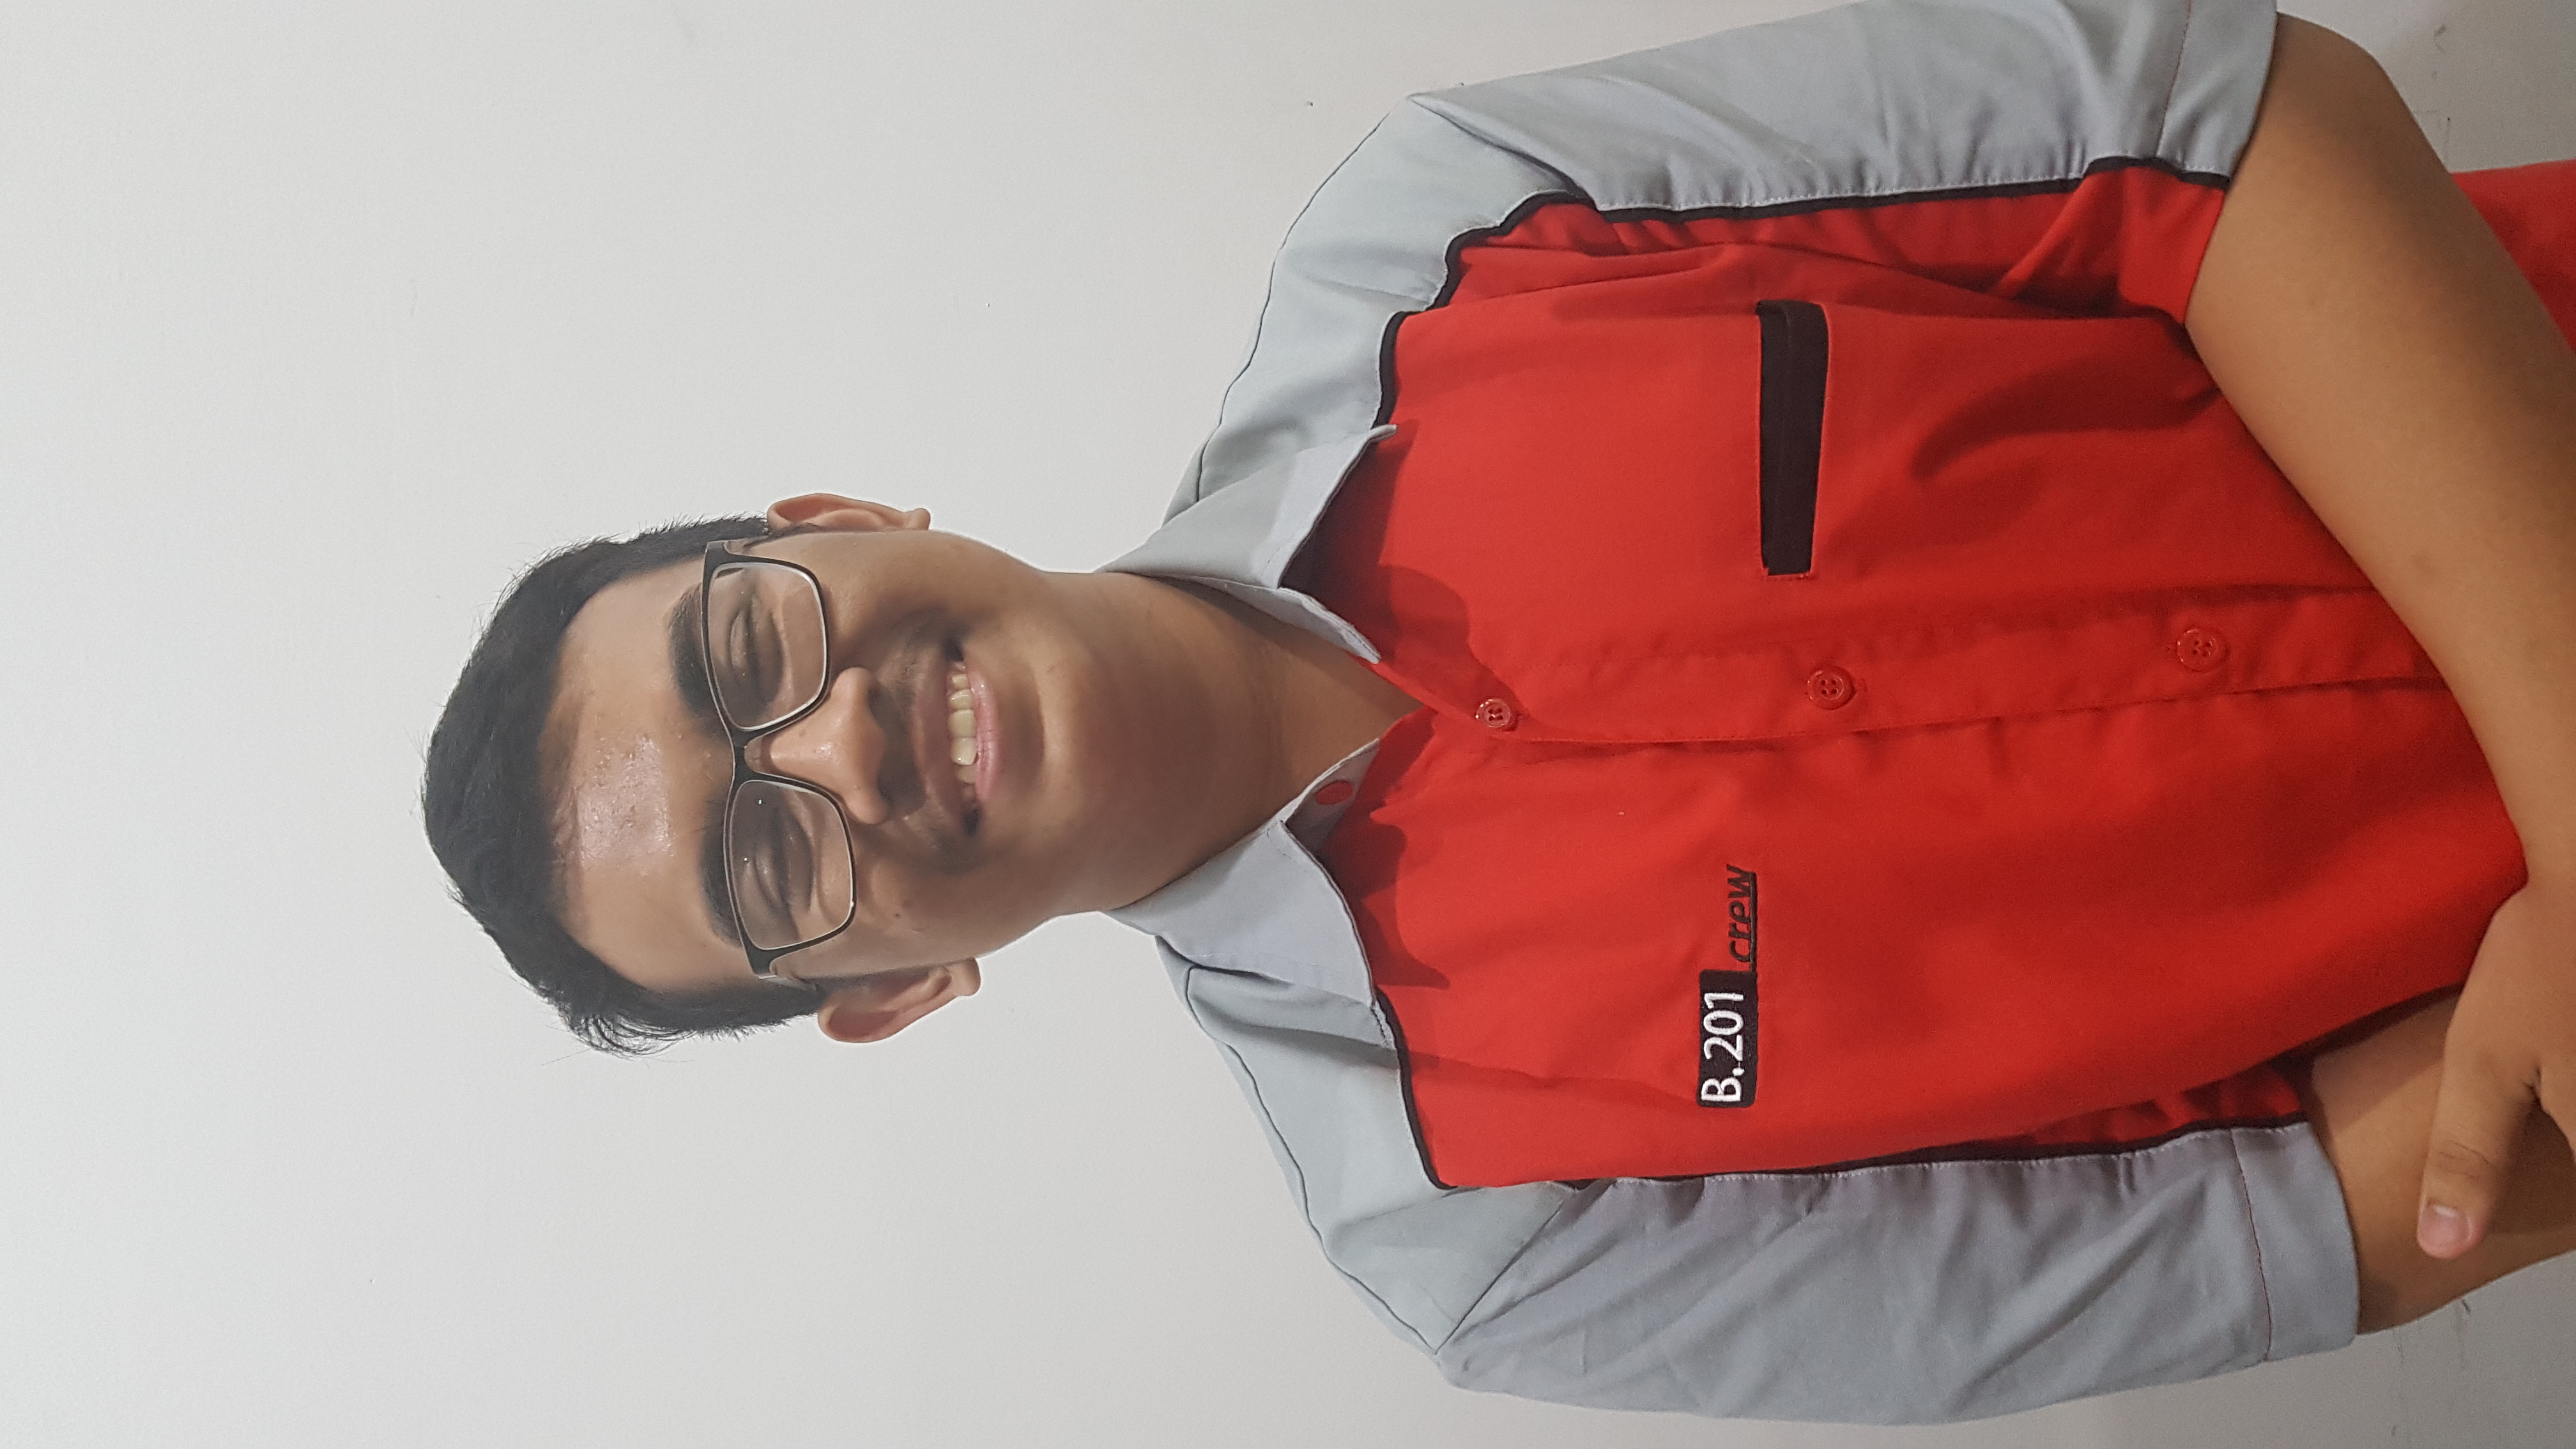
\includegraphics[width=0.5\textwidth, angle=-90]{gambar/foto.jpg}
\end{wrapfigure}

% Ubah kalimat berikut dengan biografi dari mahasiswa pertama
\noindent Aufa Nabil Amiri, lahir pada tanggal 5 Maret 2000, Surabaya. Merupakan seseorang mahasiswa yang berasal dari Institut Teknologi Sepuluh Nopember departemen Teknik Komputer. Penulis merupakan lulusan SMP Muhammadiyah 5 Surabaya dan dilanjutkan dengan SMA Negeri 2 Surabaya. Dalam masa kuliah, penulis tertarik pada bidang pengembangan \textit{Software Development}  dan Pembelajaran Mesin. Selain itu, penulis juga aktif dalam organisasi Lab B201 selama kurang 2 tahun. Penulis juga aktif dalam mengikuti kompetisi pengembangan perangkat lunak dan berhasil meraih penghargaan di ajang GEMASTIK XII 2019. Bagi pembaca yang memiliki kritik, saran, atau pertanyaan mengenai laporan magang ini dapat menghubungi penulis melalui surel aufa.nabil.amiri@gmail.com

\vspace{2ex}

% Ubah kalimat berikut dengan biografi dari mahasiswa kedua

\cleardoublepage

\end{document}
